% !TeX root = ../index.tex
\documentclass[../index.tex]{subfiles}

\begin{document}
    \section{Wykład}
        W zależności od masy ewolucja gwiazdy może przebiegać w bardzo zróżnicowany sposób. Skutkuje to różnym czasem trwania procesu i różnymi charakterystykami obiektów, na których ten proces się kończy. Do śledzenia przebiegu ewolucji gwiazdy stosuje się kilka alternatywnych sposobów:
        \begin{enumerate}
            \item \textbf{Diagram \(\log \rho_c\) – \(\log T_c\)} – obrazuje zmianę warunków panujących we wnętrzu gwiazdy pod wpływem zmiany składu chemicznego.
            \item \textbf{Diagram H-R} – ilustruje zmiany gwiazdy, które można weryfikować bezpośrednią obserwacją.
            \item \textbf{Diagram Kippenhahna} – przedstawia zmiany w całej strukturze gwiazdy w funkcji czasu.
        \end{enumerate}
        Poniżej widać diagram \(\log \rho_c\) – \(\log T_c\) z wyróżnionymi czterema obszarami, na których w jądrze panują inne równania stanu (od lewej: ciśnienie zależy od promieniowania, gaz doskonały, gaz fermiego nierelatywistyczny, gaz fermiego relatywistyczny):
        \begin{center}
            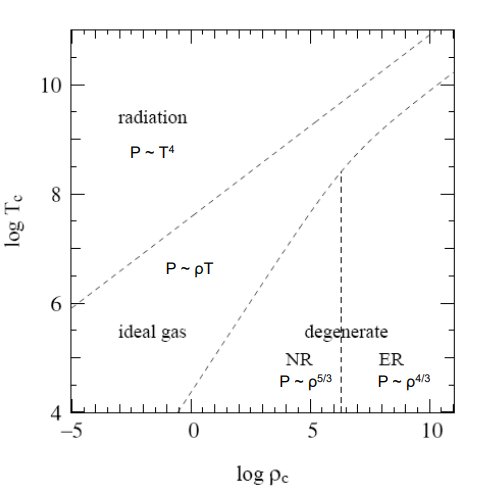
\includegraphics[width=12cm]{images/pustyLogRho_CT_C.png}
        \end{center}
        \subsection{Ewolucja gwiazd średnio masywnych}
            Poniżej widać ścieżki ewolucyjne gwiazd o masach 15, 7, 2 i 1 mas Słońca:
            \begin{center}
                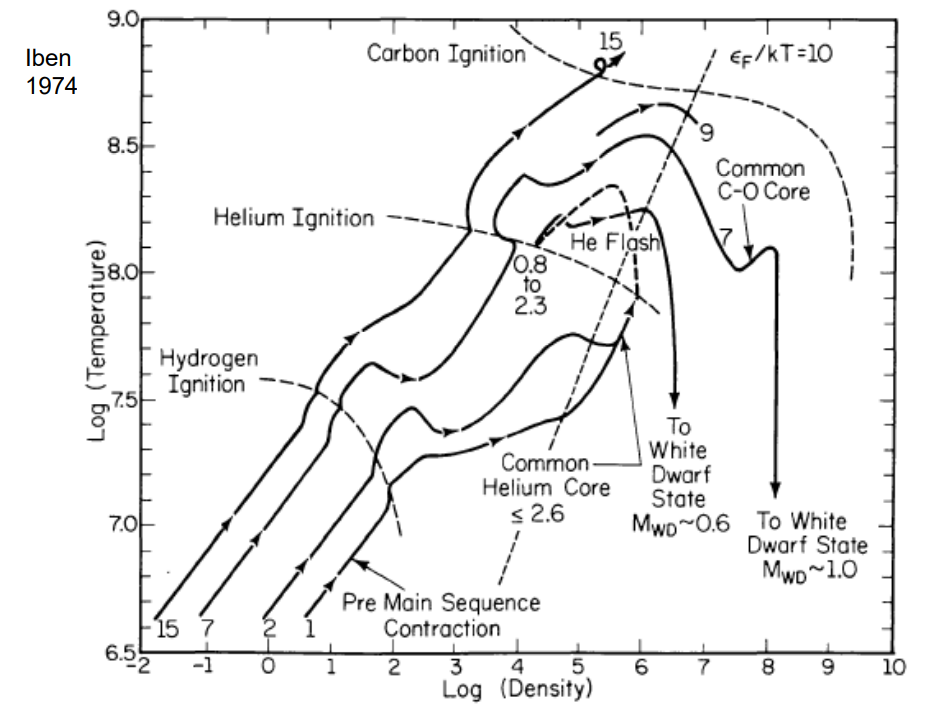
\includegraphics[width=12cm]{images/logRho_CT_C.png}
            \end{center}
            Jak widać najcięższa gwiazda w żadnym momencie nie opuszcza strefy gazu doskonałego i tylko one przekraczają linię oznaczającą zapłon węgla. Pozostałe ostatecznie skręcają w kierunku obszaru gazu zdegenerowanego, gdzie kończą jako białe karły. Gwiazdy o masach 0.8 – 2.3 mas Słońca inicjują zapłon helu w warunkach degeneracji. Dochodzi wówczas do \textbf{błysku helowego}(więcej o nim później). Gwiazdy o mniejszej masie nie zapalają helu wcale.\\
            Ilustracja poniżej pokazuje wędrówkę gwiazd po wykresie H-R w wyniku ich ewolucji:
            \begin{center}
                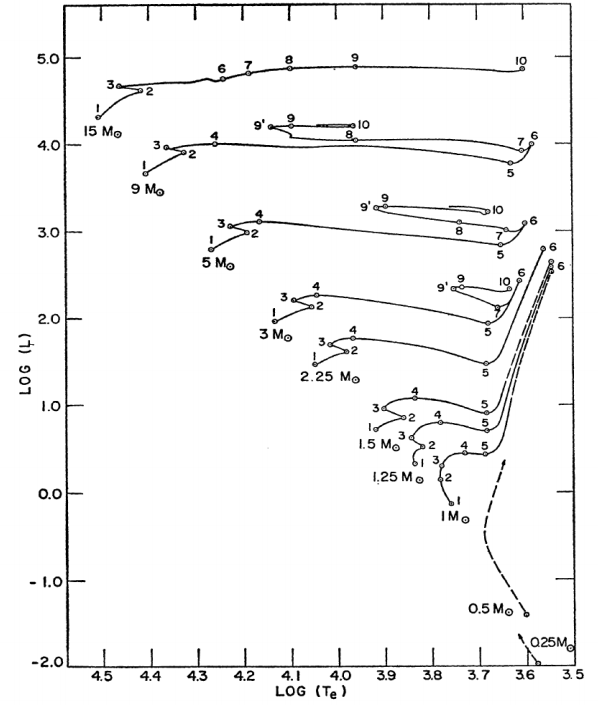
\includegraphics[width=10cm]{images/ewolucjaGwiazdHRII.png}
            \end{center}
            Liczby przy różnych krzywych odpowiadają tym samym etapom ewolucji (ale niekoniecznie temu samemu czasowi – ewolucje przebiegają w różnym tempie). Jak widać, mimo kurczenia się jądra (w celu syntezy ciężkich pierwiastków niż wodór) całkowity rozmiar gwiazdy zwiększa się (gwiazdy stają się \textbf{czerwonymi olbrzymami}). Otoczka reaguje lustrzanie do jądra – jeśli jądro się kurczy to otoczka się rozrasta i vice versa. Efekt ten spowodowany jest zmianami w energii grawitacyjnej jądra. Poniżej na wykresie Kippenhahna widać zobrazowanie tego procesu:
            \begin{center}
                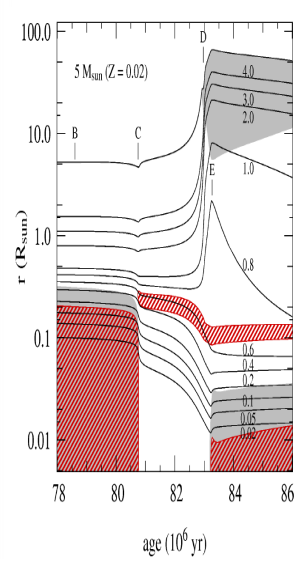
\includegraphics[width=6cm]{images/ewolucjaGwiazdKippenhahn.png}
            \end{center}
            Czerwony obszary to te, w których zachodzą reakcje jądrowe, a szare to obszary konwekcji.\\
            Do \textbf{błysku helowego} dochodzi, gdy podczas przechodzenia na spalanie helu, jądro gwiazdy jest w stanie zdegenerowanym. W przypadku degeneracji ciśnienie nie zależy od temperatury – nie działa mechanizm regulujący tempo reakcji(reakcja \(3\alpha\)). Wydzielana energia zwiększa temperaturę, co przyspiesza tempu zachodzenia tego procesu. Odpowiednio duży wzrost temperatury przy stałym ciśnieniu wywołuje zniesienie degeneracji i przejście gwiazdy w stan gazu doskonałego. W momencie błysku wydzielona jest energia 10 miliardów słońce, ale sama gwiazda przygasa, ponieważ większość tej energii konsumowana jest na likwidacje degeneracji i zwiększanie rozmiarów jądra (regulacja tempa procesu).\\
            Po przejściu na spalanie helu gwiazdy zajmują miejsce na \textbf{gałęzi horyzontalnej} wykresu H-R poruszając się w lewo, a po pewnym czasie skręcają w prawo i do góry – na tzw. \textbf{asymptotyczną gałąź olbrzymów}. W obrębie tych procesów budowa gwiazdy znacznie się zmienia:
            \begin{center}
                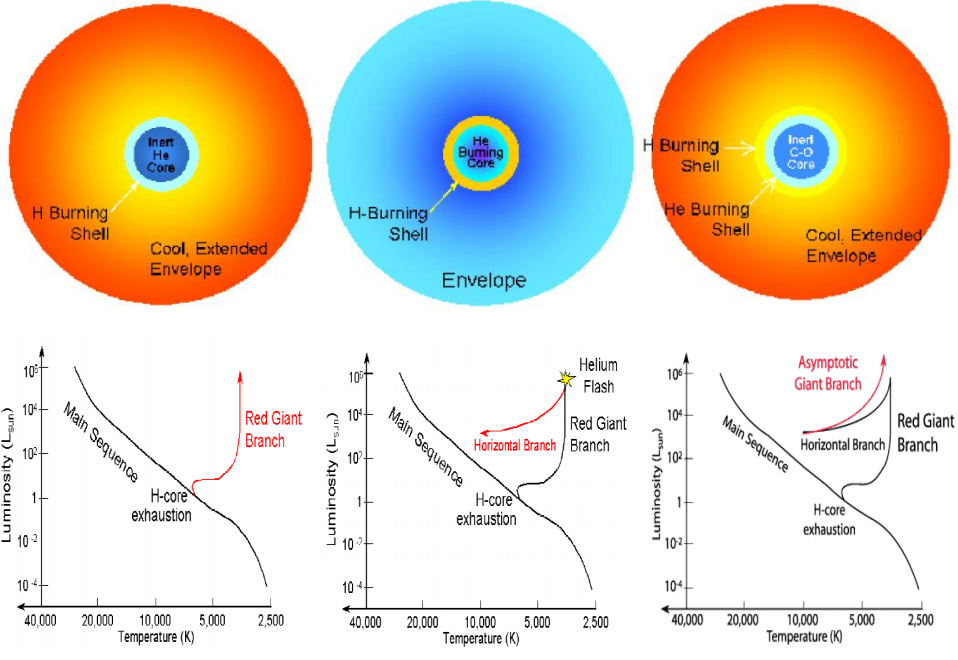
\includegraphics[width=14cm]{images/ewolucjaGwiazdOlbrzymy.png}
            \end{center}
            Na asymptotycznej gałęzi olbrzymów można wyróżnić jadro węglowo-tlenowe powłokę, w której spalany jest hel i powłokę, w której spalany jest wodór oraz otoczkę (nawet po ustaniu procesu spalania helu czy wodoru w jądrze powstają wokół niego otoczki, w których te procesy nadal zachodzą, jednocześnie będąc źródłem paliwa dla niższych warstw). W zasadzie można wyróżnić dwa różne byty – malutkie (ok 4 x promień Ziemi) jądro i bardzo rozrzedzona chmura wodoru zajmującą kulę o promieniu kilkuset większym niż Słońce.\\
            Tempo zachodzenia reakcji w obu powłokach podlega powtarzającym się zmianom. Krótkotrwałym wzrostom towarzyszy gwałtowne rozprężanie, które ogranicza tempo, po czym stopniowa kontrakcja powoduje jego zwiększenie do poziomu skutkującego kolejnym rozprężaniem warstwy. To zjawisko nazywa się \textbf{pulsami termicznymi}:
            \begin{center}
                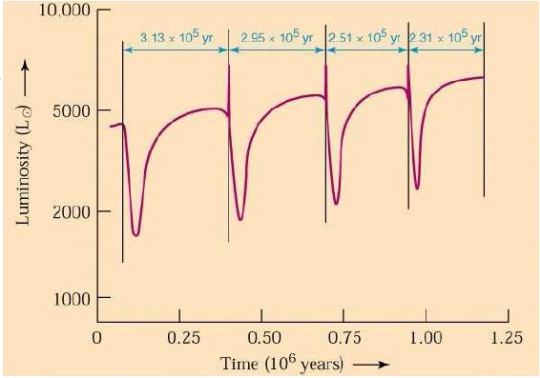
\includegraphics[width=12cm]{images/pulsyTermiczne.png}
            \end{center}
            Zaburzenia przenoszą się do otoczki, gdzie ich amplituda ulega zwiększeniu. Skutkuje to powtarzającym się odrzucaniem zewnętrznych fragmentów otoczki – powstają \textbf{mgławice planetarne}. W rezultacie przez pewien okres gwiazda staje się wielkim obłokiem rzadkiej materii z małej wielkości świecącym i gęstym jądrem wewnątrz. Po tysiącach lat obłok rozwiewa się zupełnie i jedyne co pozostaje to owo jądra – gwiazda staje się \textbf{białym karłem}.
        \subsection{Ewolucja gwiazd masywnych}
            
\end{document}